\clearpage % clear the prior chapter's page

\chapter{AlphaFold2 predicts the inward-facing conformation of the multidrug transporter LmrP} \label{app:alphafold2}
%\vspace{-7mm}
%\bigskip

The contents of this Appendix have been previously published \citep*{DelAlamo2021b}.

%\vspace{-7mm}
\bigskip

As part of the 14th annual \gls{casp}, the protein structure prediction algorithm AlphaFold2 generated multiple models of the proton/drug antiporter LmrP. Previous experimental data from \gls{deer} spectroscopy, a technique which reports distance distributions between spin labels attached to proteins, suggest that one of the lower-ranked models may have captured a conformation that has so far eluded experimental structure determination.

\begin{figure}[H]
\centering
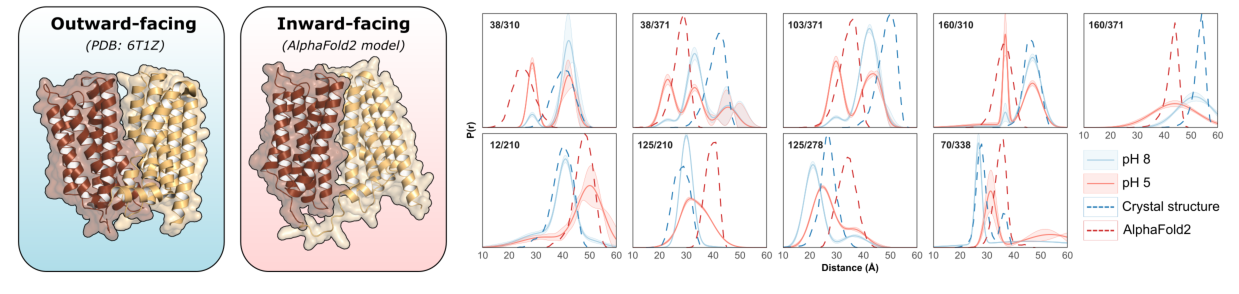
\includegraphics[width=6.5in]{Figures/lmrp_data.pdf}
 \caption[An IF model of LmrP generated by AlphaFold2 is consistent with experimental data.]{An IF model of LmrP generated by AlphaFold2 is consistent with experimental data. Left: \Gls{of} and \gls{if} conformations determined using X-ray crystallography and modeled by AlphaFold2, respectively. Right: Experimental \gls{deer} distance distributions on the extracellular and intracellular sides of the protein, respectively, overlap with distances predicted by AlphaFold2 model 1. Dashed lines are distance distributions predicted by either the crystal structure (blue) or the model (red). These data have been previously published.}
\label{fig:lmrp_data}
\end{figure}

\section{Main Text}

Active transporters such as LmrP alternate between \gls{of} and \gls{if} conformations during their transport cycles \citep*{Boudker2010, Masureel2014, Martens2016}. Whereas the crystal structure captures LmrP in the former \citep*{Debruycker2020}, AlphaFold2 modeled LmrP in the latter \citep*{Jumper2020} (Figure \ref{fig:lmrp_data}). Because LmrP is a proton/drug antiporter, we carried out \gls{deer} distance measurements \citep*{Jeschke2012, Dastvan2019, Mchaourab2011} at low and neutral pH to stabilize the \gls{if} and \gls{of} conformation, respectively (shown in red and blue in Figure \ref{fig:lmrp_data}). To evaluate the \gls{if} model's consistency with the low pH DEER data, we modeled the predicted distances \emph{in silico} using MDDS \citep*{Islam2013}, a program hosted on the CHARMM-GUI web server \citep*{Jo2014}. Not only do the predicted distances overlap remarkably well with our experimental data (Figure \ref{fig:lmrp_data}, dashed and solid lines, respectively), but importantly the magnitudes of the experimental distance changes agree with those predicted between the \gls{of} crystal structure and AlphaFold2's \gls{if} model. These results suggest that the AlphaFold2 model depicts a functionally relevant intermediate of LmrP.


\begin{wrapfigure}{r}{0.5\textwidth}
\centering
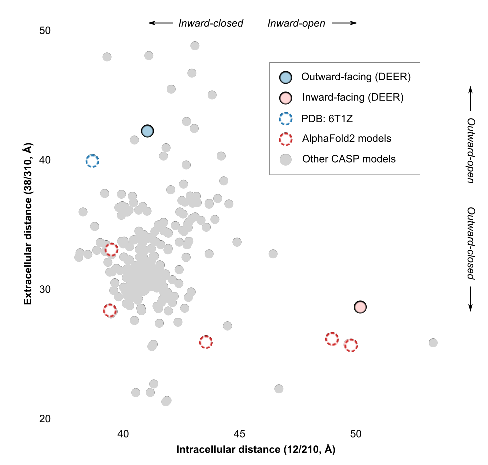
\includegraphics[width=3.25in]{Figures/lmrp_caspmodels.pdf}
 \caption[Predicted DEER distances of all CASP14 LmrP models.]{Predicted DEER distances of all CASP14 LmrP models. X and Y axes reflect the average predicted \gls{deer} distances of all \gls{casp} LmrP models on the intracellular side and extracellular sides, respectively. Solid blue and red circles represent components from the experimental \gls{deer} data corresponding to outward- and inward-facing conformations, respectively. The inward-facing AlphaFold2 model shown in panel A is located on the bottom-right.}
\label{fig:lmrp_caspmodels}
\end{wrapfigure}

The significance of this breakthrough in modeling transporter conformations is reinforced by comparison of this model to those submitted by other contestants, which overwhelmingly depicted LmrP in an occluded conformation (Figure \ref{fig:lmrp_caspmodels}). Occluded models result from methodological biases that favor compactness \citep*{Nicoludis2018}. Therefore, the success of AlphaFold2 in modeling \gls{if} LmrP suggests that these biases may finally have been overcome. Additionally, it sets the stage for the structural characterization of transporters and their functional intermediates by integrating computational modeling with experimental spectroscopy.

\section{Acknowledgments}

The work presented here was supported by the National Institutes of Health (GM077659).